\documentclass[12pt, fullpage,letterpaper]{article}

\usepackage[margin=1in]{geometry}
\usepackage{url}
\usepackage{amsmath}
\usepackage{amssymb}
\usepackage{xspace}
\usepackage{graphicx}
\usepackage{hyperref}
\usepackage{listings}

\newcommand{\semester}{Spring 2019}
\newcommand{\assignmentId}{2}
\newcommand{\releaseDate}{11 Feb, 2019}
\newcommand{\dueDate}{11:59pm, 25 Feb, 2019}

\newcommand{\bx}{{\bf x}}
\newcommand{\bw}{{\bf w}}

\title{CS 5350/6350: Machine Learining \semester}
\author{Homework \assignmentId}
\date{Handed out: \releaseDate\\
	Due: \dueDate}



% Alias for the Solution section header
\newcommand{\solution}{\textbf{\large Solution}}



\begin{document}
\maketitle

% Math commands by Thomas Minka
\newcommand{\var}{{\rm var}}
\newcommand{\Tr}{^{\rm T}}
\newcommand{\vtrans}[2]{{#1}^{(#2)}}
\newcommand{\kron}{\otimes}
\newcommand{\schur}[2]{({#1} | {#2})}
\newcommand{\schurdet}[2]{\left| ({#1} | {#2}) \right|}
\newcommand{\had}{\circ}
\newcommand{\diag}{{\rm diag}}
\newcommand{\invdiag}{\diag^{-1}}
\newcommand{\rank}{{\rm rank}}
% careful: ``null'' is already a latex command
\newcommand{\nullsp}{{\rm null}}
\newcommand{\tr}{{\rm tr}}
\renewcommand{\vec}{{\rm vec}}
\newcommand{\vech}{{\rm vech}}
\renewcommand{\det}[1]{\left| #1 \right|}
\newcommand{\pdet}[1]{\left| #1 \right|_{+}}
\newcommand{\pinv}[1]{#1^{+}}
\newcommand{\erf}{{\rm erf}}
\newcommand{\hypergeom}[2]{{}_{#1}F_{#2}}

% boldface characters
\renewcommand{\a}{{\bf a}}
\renewcommand{\b}{{\bf b}}
\renewcommand{\c}{{\bf c}}
\renewcommand{\d}{{\rm d}}  % for derivatives
\newcommand{\e}{{\bf e}}
\newcommand{\f}{{\bf f}}
\newcommand{\g}{{\bf g}}
\newcommand{\h}{{\bf h}}
%\newcommand{\k}{{\bf k}}
% in Latex2e this must be renewcommand
\renewcommand{\k}{{\bf k}}
\newcommand{\m}{{\bf m}}
\newcommand{\mb}{{\bf m}}
\newcommand{\n}{{\bf n}}
\renewcommand{\o}{{\bf o}}
\newcommand{\p}{{\bf p}}
\newcommand{\q}{{\bf q}}
\renewcommand{\r}{{\bf r}}
\newcommand{\s}{{\bf s}}
\renewcommand{\t}{{\bf t}}
\renewcommand{\u}{{\bf u}}
\renewcommand{\v}{{\bf v}}
\newcommand{\w}{{\bf w}}
\newcommand{\x}{{\bf x}}
\newcommand{\y}{{\bf y}}
\newcommand{\z}{{\bf z}}
%s\newcommand{\l}{\boldsymbol{l}}
\newcommand{\A}{{\bf A}}
\newcommand{\B}{{\bf B}}
\newcommand{\C}{{\bf C}}
\newcommand{\D}{{\bf D}}
\newcommand{\E}{{\bf E}}
\newcommand{\F}{{\bf F}}
\newcommand{\G}{{\bf G}}
\renewcommand{\H}{{\bf H}}
\newcommand{\I}{{\bf I}}
\newcommand{\J}{{\bf J}}
\newcommand{\K}{{\bf K}}
\renewcommand{\L}{{\bf L}}
\newcommand{\M}{{\bf M}}
\newcommand{\N}{\mathcal{N}}  % for normal density
%\newcommand{\N}{{\bf N}}
\renewcommand{\O}{{\bf O}}
\renewcommand{\P}{{\bf P}}
\newcommand{\Q}{{\bf Q}}
\newcommand{\R}{{\bf R}}
\renewcommand{\S}{{\bf S}}
\newcommand{\T}{{\bf T}}
\newcommand{\U}{{\bf U}}
\newcommand{\V}{{\bf V}}
\newcommand{\W}{{\bf W}}
\newcommand{\X}{{\bf X}}
\newcommand{\Y}{{\bf Y}}
\newcommand{\Z}{{\bf Z}}

% this is for latex 2.09
% unfortunately, the result is slanted - use Latex2e instead
%\newcommand{\bfLambda}{\mbox{\boldmath$\Lambda$}}
% this is for Latex2e
\newcommand{\bfLambda}{\boldsymbol{\Lambda}}

% Yuan Qi's boldsymbol
\newcommand{\bsigma}{\boldsymbol{\sigma}}
\newcommand{\balpha}{\boldsymbol{\alpha}}
\newcommand{\bpsi}{\boldsymbol{\psi}}
\newcommand{\bphi}{\boldsymbol{\phi}}
\newcommand{\boldeta}{\boldsymbol{\eta}}
\newcommand{\Beta}{\boldsymbol{\eta}}
\newcommand{\btau}{\boldsymbol{\tau}}
\newcommand{\bvarphi}{\boldsymbol{\varphi}}
\newcommand{\bzeta}{\boldsymbol{\zeta}}

\newcommand{\blambda}{\boldsymbol{\lambda}}
\newcommand{\bLambda}{\mathbf{\Lambda}}
\newcommand{\bOmega}{\mathbf{\Omega}}
\newcommand{\bomega}{\mathbf{\omega}}
\newcommand{\bPi}{\mathbf{\Pi}}

\newcommand{\btheta}{\boldsymbol{\theta}}
\newcommand{\bpi}{\boldsymbol{\pi}}
\newcommand{\bxi}{\boldsymbol{\xi}}
\newcommand{\bSigma}{\boldsymbol{\Sigma}}

\newcommand{\bgamma}{\boldsymbol{\gamma}}
\newcommand{\bGamma}{\mathbf{\Gamma}}

\newcommand{\bmu}{\boldsymbol{\mu}}
\newcommand{\1}{{\bf 1}}
\newcommand{\0}{{\bf 0}}

% \newcommand{\comment}[1]{}

\newcommand{\bs}{\backslash}
\newcommand{\ben}{\begin{enumerate}}
\newcommand{\een}{\end{enumerate}}

 \newcommand{\notS}{{\backslash S}}
 \newcommand{\nots}{{\backslash s}}
 \newcommand{\noti}{{\backslash i}}
 \newcommand{\notj}{{\backslash j}}
 \newcommand{\nott}{\backslash t}
 \newcommand{\notone}{{\backslash 1}}
 \newcommand{\nottp}{\backslash t+1}
% \newcommand{\notz}{\backslash z}

\newcommand{\notk}{{^{\backslash k}}}
%\newcommand{\noti}{{^{\backslash i}}}
\newcommand{\notij}{{^{\backslash i,j}}}
\newcommand{\notg}{{^{\backslash g}}}
\newcommand{\wnoti}{{_{\w}^{\backslash i}}}
\newcommand{\wnotg}{{_{\w}^{\backslash g}}}
\newcommand{\vnotij}{{_{\v}^{\backslash i,j}}}
\newcommand{\vnotg}{{_{\v}^{\backslash g}}}
\newcommand{\half}{\frac{1}{2}}
\newcommand{\msgb}{m_{t \leftarrow t+1}}
\newcommand{\msgf}{m_{t \rightarrow t+1}}
\newcommand{\msgfp}{m_{t-1 \rightarrow t}}

\newcommand{\proj}[1]{{\rm proj}\negmedspace\left[#1\right]}
\newcommand{\argmin}{\operatornamewithlimits{argmin}}
\newcommand{\argmax}{\operatornamewithlimits{argmax}}

\newcommand{\dif}{\mathrm{d}}
\newcommand{\abs}[1]{\lvert#1\rvert}
\newcommand{\norm}[1]{\lVert#1\rVert}

%miscellaneous symbols
\newcommand{\ie}{{{i.e.,}}\xspace}
\newcommand{\eg}{{{\em e.g.,}}\xspace}
\newcommand{\EE}{\mathbb{E}}
\newcommand{\VV}{\mathbb{V}}
\newcommand{\sbr}[1]{\left[#1\right]}
\newcommand{\rbr}[1]{\left(#1\right)}
\newcommand{\cmt}[1]{}


{\footnotesize
	Author: Cade Parkison
	
	Note: Due to time constraints, I was unable to finish getting results for all of the programming parts of this assignment. My implementations made the testing very time consuming. For bagging and random forests, it took more than 3 hours each to train the classifiers according to the specifications. Because of this, I did not get the plots that were required. I do believe my implementations are mostly correct, and I hope that by looking at my code this will be noticable. I will work much harder on future assignments to improve the quality of my results. 
}


\section{Paper Problems [40 points + 6 bonus]}
\begin{enumerate}
\item~[5 points] 
\[
m > \frac{1}{\epsilon}\big(\log(|H|) + \log\frac{1}{\delta}\big)
\]

\begin{enumerate}
	\item~[2 points]
	\begin{enumerate}
		\item~[1 point]
		
		
		An interpretation Occam's Razor principle states that given two explanations of the data, the simpler explanation is preferable. According to this, I would prefer hypothesis with the smaller hypothesis space size, $H_2$. This is in line with the goal of Machine learning, to find the simplest hypothesis that is consistent with the sampled data. 
		
		
		\item~[1 point] 
		
	If we assume fixed error and confidence parameters ($\delta$ and $\epsilon$) for both learning algorithms, algorithm $L_1$ will require more samples ($m_1$) in order to produce the same error and confidence levels. This can be seen in the following inequalities: 	
	
	\[
		m_1 > \frac{1}{\epsilon}\big(\log(|H_1|) + \log\frac{1}{\delta}\big)
	\]
	
	\[
		m_2 > \frac{1}{\epsilon}\big(\log(|H_2|) + \log\frac{1}{\delta}\big)
	\]
	
	Using the inequality $|H_1| > |H_2|$, and since $\delta$ and $\epsilon$ are constant:
	
	\[
		\begin{split}
			 \frac{1}{\epsilon}\big(\log(|H_1|) + \log\frac{1}{\delta}\big) &> \frac{1}{\epsilon}\big(\log(|H_2|) + \log\frac{1}{\delta}\big)
			 \\
			 m_1 &> m_2
		\end{split}
	\]
	
	This means that if both algorithms use the same number of training samples during the learning phase, algorithm $L_2$ will have higher accuracy ($1-\epsilon$) and confidence ($1-\delta$). I therefore prefer the hypothesis with the smaller hypothesis space, $H_2$.
	
	\end{enumerate}
	
	
	
	\item~[3 points] 
	
	Using the given confidence and accuracy values, we have $\delta=0.05$ and $\epsilon=0.1$. Plugging in these as well as $|H_1|=3^{10}$, we can plug them into the original inequality to solve for $m_1$.
	
	\[
		\begin{split}
			m_1 &> 10\big(\log(3^{10}) + \log20\big)
			\\
			&> 60.72
		\end{split}	
	\]
	
	Therefore, we need at least 61 training examples to get the hypothesis with desired performance in $L_1$.
\end{enumerate}

\item~[7 points] 
\begin{enumerate}
	\item~[1 points] Simple disjunctions out of $n$ binary variables
	
		The size of the hypothesis space of boolean disjuntions is $3^n$. This is definitely PAC learnable, as seen in the previous problem with n=10.
	
	\item~[1 points] $m$-of-$n$ rules (Note that $m$ is a fixed constant).  
	
	
	\item~[1 points] General conjunctions out of $n$ binary variables (``General'' means that negations are allowed to operator on each variable before the conjunction).
	
	For purely conjunctive concepts, the hypotheses space is $3^n$, since each attribute can be required to be true, false, or just ignored. 
	
	
	\item~[2 points] General Boolean functions of $n$ binary variables. 
	
	For general boolean functions, the size of the hypothesis space is $2^{2^n}$. As n increases, this would get exponentially harder to be PAC learnable, but still possible with enough training examples. 
	
	
	\item~[2 points] Can ID3 algorithm \textit{efficiently} PAC learn the above concept classes? 
	
	ID3 would not be able to efficiently learn all these classes, due to the exponential nature of the their PAC functions. The most simple of the classes would be efficiently learnable, but not the more general cases. 
	
	
\end{enumerate}

\item~[5 points] In our lecture about AdaBoost algorithm, we introduced the definition of weighted error in each round $t$, 
\[
\epsilon_t = \frac{1}{2} - \frac{1}{2}\big(\sum_{i=1}^m D_t(i) y_i h_t(x_i)\big)
\]
where $D_t(i)$ is the weight of $i$-th training example, and $h_t(x_i)$ is the prediction of the weak classifier learned round $t$. Note that both $y_i$ and $h_t(x_i)$ belong to $\{1, -1\}$. Prove that equivalently,
\[
\epsilon_t = \sum_{y_i \neq h_t(x_i)} D_t(i).
\]

\solution

	Starting with the following definition of $Z_t$, I then take the derivative w.r.t. $\alpha_t$ and set equal to zero:
	
	\[
		\begin{split}
			Z_t = \sum_{i:h_t(x_i)=y_i} D_t(i)e^{-\alpha_t} + 	\sum_{i:h_t(x_i)\neq y_i} D_t(i)e^{\alpha_t}		
		\end{split}	
	\]
	
	\[
		\begin{split}
			\frac{dZ_t}{d\alpha_t} &= \sum_{i:h_t(x_i)=y_i} - D_t(i)e^{-\alpha_t} + 	\sum_{i:h_t(x_i)\neq y_i} D_t(i)e^{\alpha_t} = 0		
		\end{split}	
	\]
	
	\[
		\begin{split}
			 \sum_{i:h_t(x_i)=y_i} D_t(i) = 	\sum_{i:h_t(x_i)\neq y_i} D_t(i)e^{2\alpha_t} 
		\end{split}	
	\]
	
	Then, by definition and the proof proof presented in class, the error can be written as:
	
	\[
		\epsilon_t = \sum_{y_i \neq h_t(x_i)} D_t(i).
	\]
	


	\item~[8 points] 
	\begin{enumerate}
		\item~[1 point] $f(x_1, x_2, x_3) = x_1 \lor x_2 \lor x_3$
		
			Starting with the generic hyperplane formula for three dimensions, we can solve for the bias and weights to fit the above boolean disjunction.
			
			\[
				\begin{split}
					b + w_1 x_1 + w_2 x_2 + w_3 x_3 = 0
				\end{split}
			\]
			
			where $\w = [1, 1, 1]$ and $b=-1$. Putting this together gives the following linear classifier:
			
			\[
				\begin{split}
					x_1 + x_2 + x_3 \geq 1
				\end{split}
			\]
			
			This means that $f(x_1, x_2, x_3) = 1$ iff the above inequality is true. The separating hyperplane is therefore:
			
			\[
				\begin{split}
					x_1 + x_2 + x_3 - 1  = 0
				\end{split}
			\]
			
			
			

		
		\item~[1 point] $f(x_1, x_2, x_3) = x_1 \land \neg x_2 \land \neg x_3$
		
		Just as the problem above:
		
			\[
				\begin{split}
					b + w_1 x_1 + w_2 x_2 + w_3 x_3 = 0
				\end{split}
			\]
			
			where $\w = [1, -1, -1]$ and $b=-1$. Putting this together gives the following linear classifier:
			
			\[
				\begin{split}
					x_1 - x_2 - x_3 \geq 1
				\end{split}
			\]
			
			The separating hyperplane is therefore:
			
			\[
				\begin{split}
					 x_1 - x_2 - x_3 - 1  = 0
				\end{split}
			\]
		
		
		\item~[1 point] $f(x_1, x_2, x_3) = \neg x_1 \lor \neg x_2 \lor \neg x_3$ 
		
		Using De Morgan's law, the negation of a conjuntion is the disjuntion of the negations. We can therefore rewrite the above equation as:
		
			\[
				\begin{split}
					f(x_1, x_2, x_3) &= \neg x_1 \lor \neg x_2 \lor \neg x_3
					\\
					&= \neg ( x_1 \land  x_2 \land  x_3 )
				\end{split}
			\]
			
			Solving for the weights and bias gives the following:
			
			\[
				\begin{split}
					b + w_1 x_1 + w_2 x_2 + w_3 x_3 = 0
				\end{split}
			\]
			
			where $\w = [1, 1, 1]$ and $b=-3$. Putting this together gives the following linear classifier:
			
			\[
				\begin{split}
					x_1 + x_2 + x_3 < 3
				\end{split}
			\]
			
			This means that $f(x_1, x_2, x_3) = 1$ iff the above inequality is true. The separating hyperplane is therefore:
			
			\[
				\begin{split}
					 x_1 + x_2 + x_3 - 3  = 0
				\end{split}
			\]
			
			Comparing $f(x_1, x_2, x_3) = \neg ( x_1 \land  x_2 \land  x_3 )$ and $f(x_1, x_2, x_3) =  ( x_1 \land  x_2 \land  x_3 )$, the only difference is in this case we use a $<$ instead of $\geq$.
		
		
		
		\item~[2 points] $f(x_1, x_2, x_3, x_4) = (x_1 \lor x_2) \land (x_3 \lor x_4)$
		
		
		\item~[2 points] $f(x_1, x_2, x_3, x_4) = (x_1 \land x_2) \lor (x_3 \land x_4)$
		
		
		\item~[1 point] What do you conclude about the expressiveness of decision trees and linear classifiers? Why?
		
		Decision trees are able to represent any boolean functions, while linear classifiers can only represent certain subsets of boolean functions that are linearly separable. 
		
	\end{enumerate}
		
	
	\item~[6 points] The following boolean functions cannot be represented by linear classifiers. Can you work out some feature mapping such that, after mapping all the inputs of these functions into a higher dimensional space, you can easily identify a hyperplane that separates the inputs with different corresponding boolean function values? Please write down the separating hyperplane as well. 
	\begin{enumerate}
		\item $f(x_1, x_2) = (x_1 \land \neg x_2) \lor (\neg x_1 \land x_2) $
		\item $f(x_1, x_2) = (x_1 \land x_2) \lor (\neg x_1 \land \neg x_2)$
		\item $f(x_1, x_2, x_3)$ is listed in the following table
		\begin{table}[h]
			\centering
			\begin{tabular}{ccc|c}
				$x_1$ & $x_2$ & $x_3$ &  $f(x_1, x_2, x_3)$\\ 
				\hline\hline
				0 & 0 & 0 & 0 \\ \hline
				0 & 0 & 1 & 1 \\ \hline
				0 & 1 & 0 & 1 \\ \hline
				1 & 0 & 0 & 1 \\ \hline
				0 & 1 & 1 & 0\\ \hline
				1 & 1 & 0 & 0\\ \hline
				1 & 0 & 1 & 0\\ \hline
				1 & 1 & 1 & 1\\ \hline
			\end{tabular}
		\end{table}
	\end{enumerate}
	
	\item~[\textbf{Bonus}]~[6 points]  Given two vectors $\x = [x_1,  x_2]$ and $\y=[y_1,  y_2]$, find a feature mapping $\phi(\cdot)$ for each of the following functions, such that the function is equal to the inner product between the mapped feature vectors, $\phi(\x)$ and $\phi(\y)$. For example, $(\x^\top \y)^0 = \phi(\x)^\top \phi(\y)$ where $\phi(\x) = [1]$ and $\phi(\y) = [1]$; $(\x^\top \y)^1 = \phi(\x)^\top \phi(\y)$ where $\phi(\x) = \x$ and $\phi(\y) = \y$. 
	\begin{enumerate}
		\item~[2 points] $(\x^\top \y)^2$
		\item~[2 points] $(\x^\top \y)^3$
		\item~[2 points] $(\x^\top \y)^k$ where $k$ is  any positive integer.  
	\end{enumerate}

\item~[9 points] Suppose we have the training data shown in Table \ref{tb:1}, from which we want to learn a linear regression model, parameterized by a weight vector $\w$ and a bias parameter $b$.  
\begin{table}
	\centering
	\begin{tabular}{ccc|c}
		$x_1 $ & $x_2$ & $x_3$ &  $y$\\ 
		\hline\hline
		1 & -1 & 2 & 1 \\ \hline
		1 & 1 & 3 & 4 \\ \hline
		-1 & 1 & 0 & -1 \\ \hline
		1 & 2 & -4 & -2 \\ \hline
		3 & -1 & -1 & 0\\ \hline
	\end{tabular}
	\caption{Linear regression training data.}\label{tb:1}
\end{table}

\begin{enumerate}
	\item~[1 point] Write down the LMS (least mean square) cost function $J(\w, b)$. 
	
	Starting with basic cost function and expanding we get:
	
	\[
		\begin{split}
			J(\w) = \frac{1}{2} \sum_{i=1}^m (y_i - \w^T\x_i)^2
		\end{split}
	\] 
	
	\[
		\begin{split}
			J(\w, b) &= \frac{1}{2} \big(  (y_1 - (w_1x_{11} + w_2x_{12} + w_3x_{13} + b))^2 + (y_2 - (w_1x_{21} + w_2x_{22} + w_3x_{23} + b))^2 + ... \big)\\
			&= \frac{1}{2} \big((1-(w_1-w_2+2w_3+b))^2+(4-(w_1+w_2+3w_3+b))^2+(-1-(-w_1+w_2+b))^2+(-2-(w_1+2w_2-4w_4+b))^2+(3w_1-w_2-w_3+b)^2   \big)
		\end{split}
	\]
	
	
	\item~[3 points] Calculate the gradient $\frac{\nabla J}{\nabla \w}$ and $\frac{\nabla J}{\nabla b}$ 
	\begin{enumerate}
		\item when $\w = [0,0,0]^\top$ and $b = 0$;
		
		\[
			\begin{split}
				\frac{\delta J}{\delta b} &= (1-0) + (4-0) + (-1-0) + (-2-0)+ (0-0)\\
					&= 1 + 4 - 1 - 2\\
					&= 2
			\end{split}
		\]
		
		\[
			\begin{split}
				\frac{\delta J}{\delta w_1} &= (1-0)(1) + (4-0)(1) + (-1-0)(-1) + (-2-0)(1)+ (0-0)(3)\\
					&= 1 + 4 + 1 - 2\\
					&= 4
			\end{split}
		\]
		
		\[
			\begin{split}
				\frac{\delta J}{\delta w_2} &= (1-0)(-1) + (4-0)(1) + (-1-0)(1) + (-2-0)(2)+ (0-0)(-1)\\
					&= -1 + 4 -1 - 4\\
					&= -2
			\end{split}
		\]
		
		\[
			\begin{split}
				\frac{\delta J}{\delta w_3} &= (1-0)(2) + (4-0)(3) + (-1-0)(0) + (-2-0)(-4)+ (0-0)(-1)\\
					&= 2 + 12 + 0 - 8\\
					&= 6
			\end{split}
		\]
		
		\item when $\w = [-1,1,-1]^\top$ and $b = -1$;
		
		Using the same formulas as above, I got the following results:
		
		\[
				\frac{\delta J}{\delta b} = 10
		\]
		
		\[
				\frac{\delta J}{\delta w_1} = 22
		\]
		
		\[
				\frac{\delta J}{\delta w_2} = -16
		\]
		
		\[
				\frac{\delta J}{\delta w_3} = 56
		\]
		
		\item when $\w = [1/2,-1/2,1/2]^\top$ and $b = 1$..
		
		\[
				\frac{\delta J}{\delta b} = -4.5
		\]
		
		\[
				\frac{\delta J}{\delta w_1} = -7.5
		\]
		
		\[
				\frac{\delta J}{\delta w_2} = 4.0
		\]
		
		\[
				\frac{\delta J}{\delta w_3} = 5.0
		\]
		
	\end{enumerate}
	\item~[2 points] What are the optimal $\w$ and $\b$ that minimize the cost function? 
	
	Using $A^tA x = A^tb$ where A is the features and b is the outcomes, solving for x (weights), I got the following:
	
	\[
		b = -1
	\]

	\[
		\w = [1, 1, 1]
	\]	
	
	\item~[3 points] Now, we want to use stochastic gradient descent to minimize $J(\w, b)$. We initialize $\w = \0$ and $b = 0$. We set the learning rate $r = 0.1$ and sequentially go through the $5$ training examples. Please list the stochastic gradient in each step and the updated $\w$ and $b$.  
\end{enumerate}
\end{enumerate}

\section{Practice [60 points + 10 bonus]}
\begin{enumerate}
	\item~[2 Points] Update your machine learning library. Please check in your implementation of decision trees in HW1 to your GitHub repository. Remember last time you created a folder ``Decision Tree". You can commit your code into that folder. Please also supplement README.md with concise descriptions about how to use your code to learn decision trees (how to call the command, set the parameters, etc). Please create two folders ``Ensemble Learning" and ``Linear Regression''  in the same level as the folder ``Decision Tree''.  


\item~[36 points] We will implement the boosting and bagging algorithms based on decision trees.  Let us test them on the bank marketing dataset in HW1 (bank.zip in Canvas). We use the same approach to convert the numerical features into binary ones. That is, we choose the media (NOT the average) of the attribute values (in the training set) as the threshold, and examine if the feature is bigger (or less) than the threshold.  For simplicity, we treat ``unknown'' as a particular attribute value, and hence we do not have any missing attributes for both training and test.
\begin{enumerate}
	\item~[8 points] 
	
	
	Adaboost greatly improves on the results of a single fully expanded decision tree by averaging the results of many decision stump models. In my implementation, I ran into the problem where after 2 iterations, all of the errors were stuck at a constant value of around 0.002. I believe this had to do with the way I implemented the alpha and epsilon calculations. The epsilon values started over 0.5 and converged to 0.5, which caused my alphas to go to zero. When all the alphas were zero, the weights never changed and the errors remained constant. If I had more time on the assignment, I believe this issue could be fixed.
	
	\item~[8 points] Based on your code of the decision tree learning algorithm (with information gain), implement a Bagged trees learning algorithm. Note that each tree should be fully expanded --- no early stopping or post pruning. Vary the number of trees from $1$ to $1000$, report how the training and test errors vary along with the tree number in a figure. Overall, are bagged trees better than a single tree? Are bagged trees better than Adaboost? 
	
	
	For the bagged trees implementation, my algorithm took multiple hours to run to the desired 1000 trees. Because of this, I was unable to get a good plot of errors vs trees. But, when testing on a small number of trees, the result was a decrease in error over time. This appeared to be better than a single tree. As expected, this method decreases the variance of the predictions. Compared to Adaboost, this algorithm performed worse, but both algorithms were better than a single decision tree. Overall, I think boosting would preform better in most cases. 

	\item~[6 points] 
		
		Unfortunately, due to time constraints I was unable to complete this part of the assignment. 

	 
	\item~[8 points] Implement the random forest algorithm as we discussed in our lecture. Vary the number of random trees from $1$ to $1000$. Note that you need to modify your tree learning algorithm to randomly select a subset of features before each split. Then use the information gain to select the best feature to split.  Vary the size of the feature subset from $\{2, 4, 6\}$. Note that if your feature subset happen to be all the features used before, simply resample the subset.  Report in a figure how the training and test errors vary along with the number of random trees for each feature subset size setting. How does the performance compare with bagged trees? 
	
	\item~[6 points] Following (c), estimate the bias and variance terms, and the squared error for a single random tree and the whole forest.  Comparing with the bagged trees, what do you observe? What can you conclude? 
\end{enumerate}

\item~[\textbf{Bonus}][10 points] In practice, to confirm the performance of your algorithm, you need to find multiple datasets for test (rather than one). You need to extract and process data by yourself. Now please use the credit default dataset in UCI repository \href{https://archive.ics.uci.edu/ml/datasets/default+of+credit+card+clients}{https://archive.ics.uci.edu/ml/datasets/default+of+credit+card+clients}. Randomly choose $24000$ examples for training and the remaining $6000$ for test. Feel free to deal with continuous features. Run bagged trees, random forest, and Adaboost with decision stumps algorithms for $1000$ iterations. Report in a figure how the training and test errors vary along with the number of iterations, as compared with a fully expanded single decision tree. Are the results consistent with the results you obtained from the bank dataset?

	\item~[22 points] We will implement the LMS method for a linear regression task. The dataset is from UCI repository (\url{https://archive.ics.uci.edu/ml/datasets/Concrete+Slump+Test}). The task is to predict the real-valued SLUMP of the concrete, with $7$ features. The features and output are listed in the file ``concrete/data-desc.txt''. The training data are stored in the file ``concrete/train.csv'', consisting of $53$ examples. The test data are stored in ``concrete/test.csv'', and comprise of $50$ examples. In both the training and testing datasets, feature values and outputs are separated by commas. 
	
	\begin{enumerate}
		\item~[8 points] 
		
		
		When implementing Batch Gradient Descent, I started with learning rate of 1 and slowly decreased it until the algorithm converged. I found this convergence happened around a learning rate of $r=0.01$. At this rate, my algorithm starts to converge very quickly, at about 1000 iterations. I also found that by initializing the weight vector to 1 instead of 0, the algorithm converged much faster.
		
		The learned weight vector is the following:
		
		\[
			\w =  [-0.01520,0.90022,0.78594,0.8506, 1.29862,0.12983,  1.5717 ,  0.99834] 
		\]
		
		Using this weight vector to calculate the cost function value of the test data, I get a function value of $23.361$.
		
		The figure below shows the convergence of the cost function vs time.
		
		
		
		
		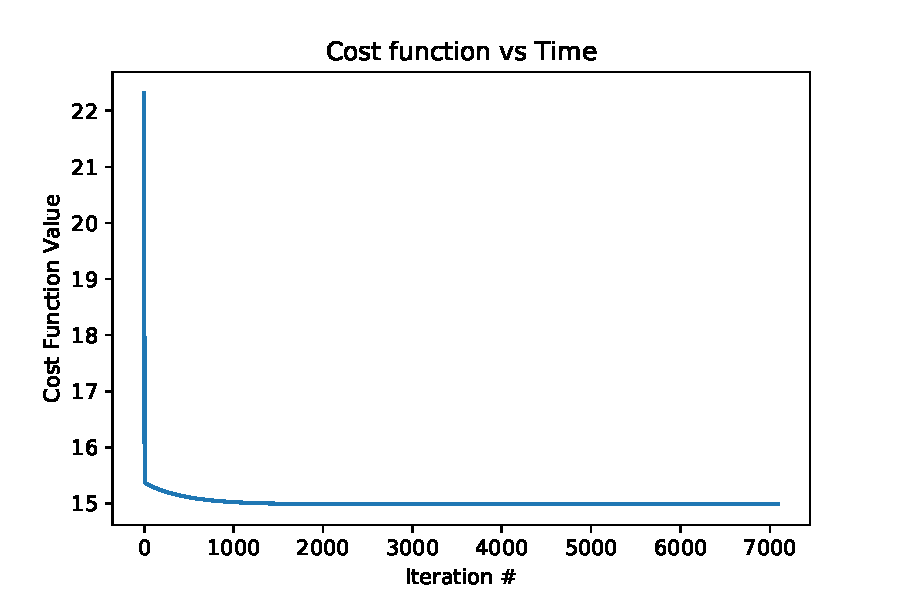
\includegraphics{BGD_cost_vs_time.pdf}
		
 
		\item~[8 points] Implement the stochastic gradient descent (SGD) algorithm. You can initialize your weight vector to be $\0$. Each step, you randomly sample a training example, and then calculate the stochastic gradient to update the weight vector.  Tune the learning rate $r$ to ensure your SGD converges. To check convergence, you can calculate the cost function of the training data after each stochastic gradient update, and draw a figure showing how the cost function values vary along with the number of updates. At the beginning, your curve will oscillate a lot. However, with an appropriate $r$, as more and more updates are finished, you will see the cost function tends to converge. Please report the learned weight vector, and the learning rate you chose, and the cost function value of the test data with your learned weight vector.   
		
		For stochastic gradient descent, I started with the learning rate used in batch gradient descent, $r=0.01$, and calculated the cost function vs the number of updates. With this learning rate, the cost fluctuated a lot. This can be seen in the figure below.
		
		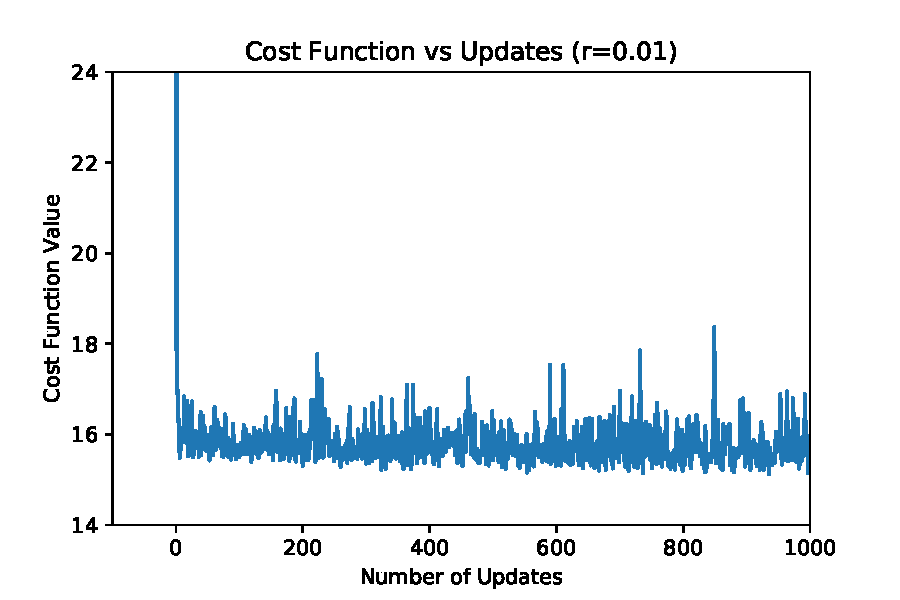
\includegraphics{r01.pdf}
		
		Next, I started to lower the learning rate and compare the plots. Below are the plots for learning rates of 0.005, 0.001, 0.0005, and 0.0001. As the learning rates decrease, the number of updates required for convergence increases. Also, the plots get much smoother, as can be seen below. 
		
		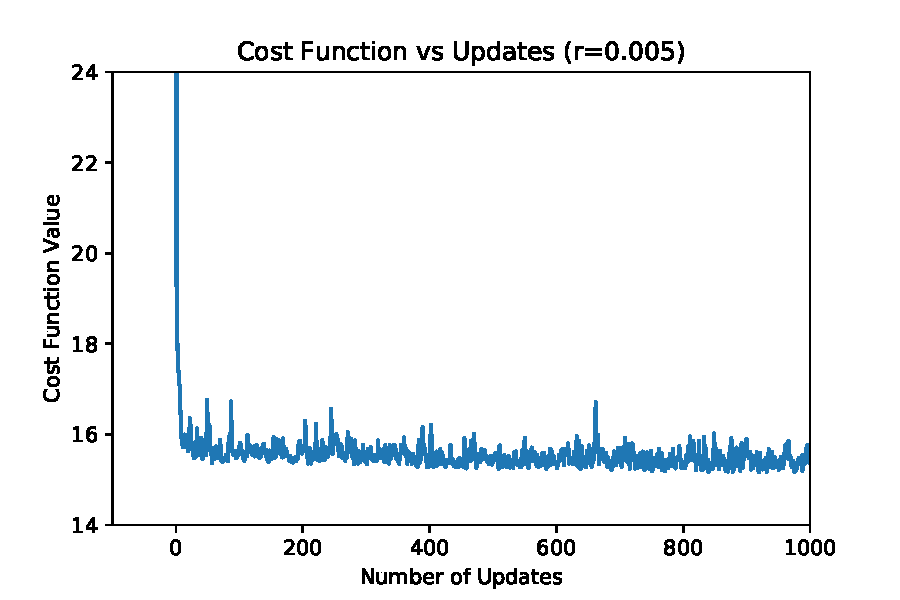
\includegraphics{r005.pdf}
		
		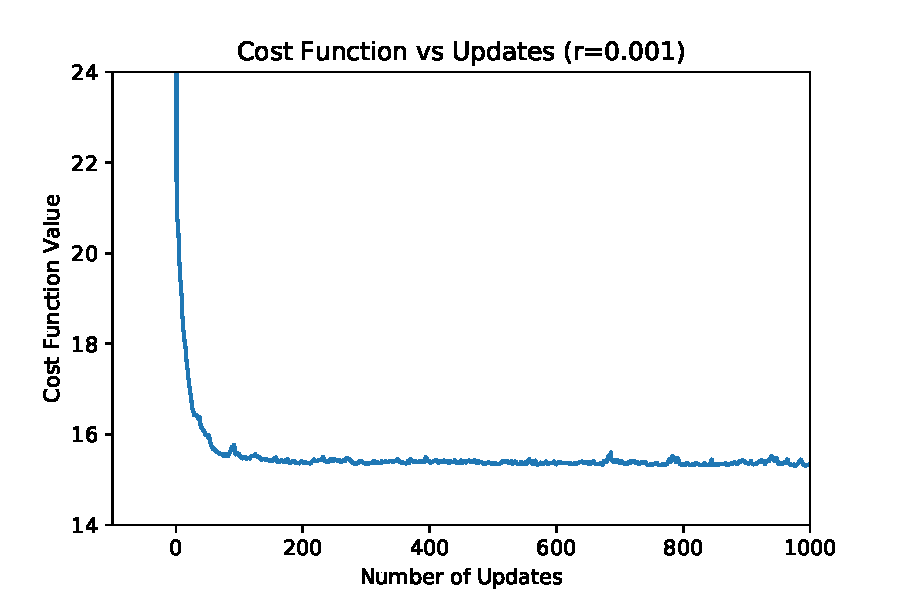
\includegraphics{r001.pdf}
		
		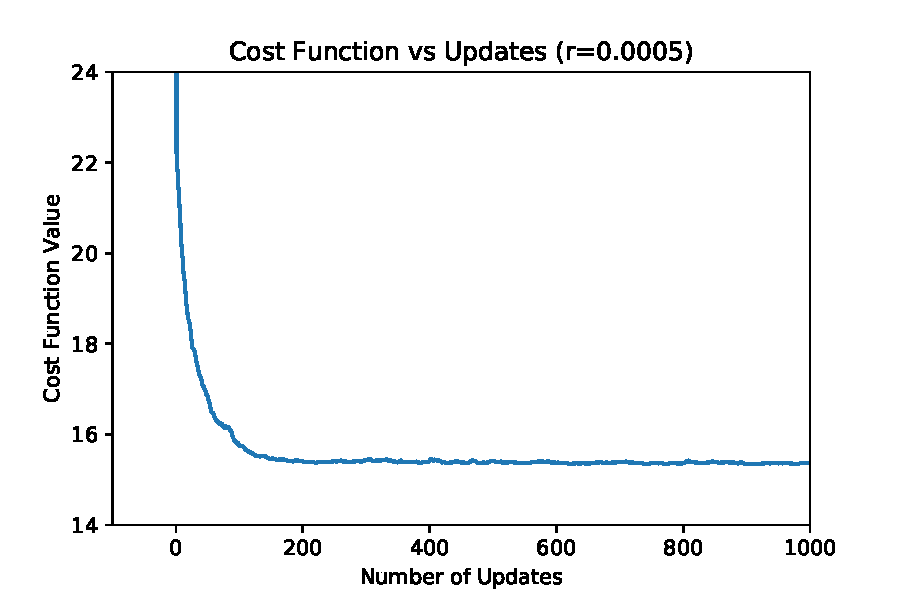
\includegraphics{r0005.pdf}
		
		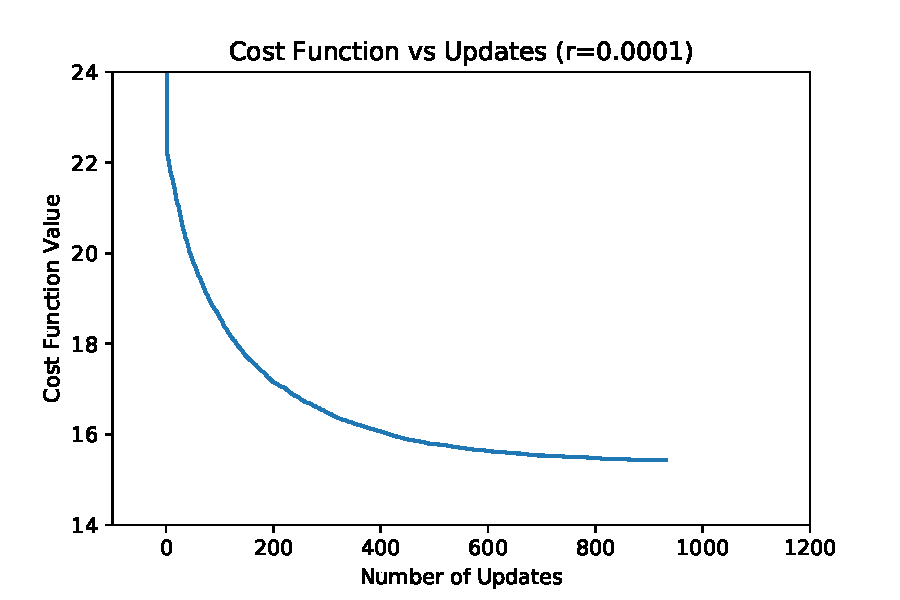
\includegraphics{r0001.pdf}
		
		From the plots above, it appears a learning rate between 0.0005 and 0.0001 will provide a constant steady state value while also converging quickly. 
		
		For the learning rate of 0.0001, the weight vector calculated is the following:
		
		\[
			\w =  [-0.03712, -0.05441, -0.22296, -0.2290 ,  0.45588, -0.03449,  0.20263, -0.01664]
		\]
		
		Using this weight vector, I calculated the cost function of the test data to be $f=22.415$, which is fairly close to the cost value using batch gradient descent.
		
		\item~[6 points] We have discussed how to  calculate the optimal weight vector with an analytical form. Please calculate the optimal weight vector in this way. Comparing with the  weight vectors learned by batch gradient descent and stochastic gradient descent, what can you conclude? Why?
		
		I calculated the analytical form of the weight vector with the following equation:
		
		\[
			A^tA x = A^tb
		\]
		
		where x is the weight vector, A is the feature matrix, and b is the output vector. Solving for x (w), the resulting weights are:
		
		\[
			\w =  [ 0.03833, -1.05154, -1.38454, -1.0843, -0.34476, -0.24711, -1.36924, -0.65715]
		\]
		
		
		Calculating the cost of the training data gives $f=25.75$. Using this weight vector to calculate cost of the test data, I get $f=15.4873$. This value is very close to the converging cost in both BGD and SGD algorithms. Comparing the three weight vectors, all weights are very different. Even though the various weights are different, the calculated costs seem to be similar. In conclusion, I can say that both batch gradient descent and stochastic gradient descent are good at fitting to the training data, but not great at generalizing. 
		
		
		
			
		
	\end{enumerate}

\end{enumerate}

\end{document}
%%% Local Variables:
%%% mode: latex
%%% TeX-master: t
%%% End:
